\documentclass[12pt]{beamer}
\title[COJ:Java:03]{JPL :: Command-Line Arguments}
\author[TS]{TalentSprint}
\institute[L\&D]{Licensed To Skill}
\date{Version 1.0.4}
\usefonttheme{serif}
\usecolortheme{orchid}
\usepackage{bookman}
\usepackage{hyperref}
\usepackage[T1]{fontenc}
\usepackage{color}
\usepackage{graphicx}
\usepackage{listings}
\graphicspath{{../../Images/}}
\usepackage{tikz}
\beamertemplateballitem
\usebackgroundtemplate{
\includegraphics[width=\paperwidth]{TS-XP-Logo.jpg}}
\lstset{language=Java,numbers=left, numberstyle=\tiny, basicstyle=\footnotesize, numbersep=10pt, showstringspaces=false, breaklines=true,keepspaces=true, columns=flexible}
\begin{document}

\begin{frame}
  \titlepage
\end{frame}

\begin{frame}{Learning Objectives}
The content in this presentation is aimed at teaching learners to:
  \begin{itemize}
  \item Explain programming thinking
  \item Explain the fundamental elements of programming
  \item Use command-line arguments in Java programs
  \item Explain common errors associated with command-line arguments
  \end{itemize}
\end{frame}

\begin{frame}{Command-Line Arguments}
\begin{figure}[H]
  \begin{center}
   
\includegraphics[scale=.4]{program-thinking.png}
  \end{center}
 \end{figure}
 \end{frame}
 
\begin{frame}{Command-Line Arguments}
 \begin{figure}[H]
  \begin{center}
   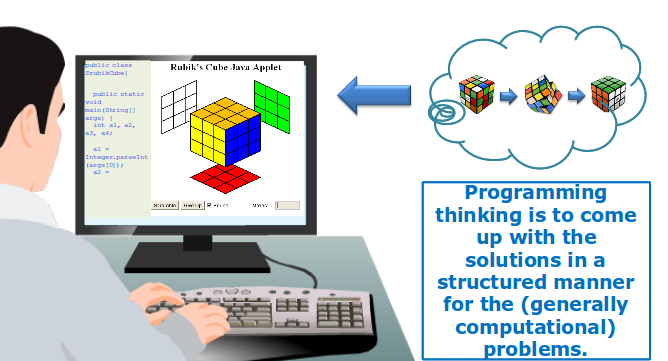
\includegraphics[scale=.4]{programming-thinking.png}
  \end{center}
 \end{figure}
\end{frame}

\begin{frame}{Command-Line Arguments}
 \textbf{Let's think}
 \begin{description}
  \item [Problem] Find sum of four given numbers.
  \item [High Level  Solution] Find the sum by considering one number at a time and adding it to the sum.
  \item [Detailed Solution]\
  \begin{itemize}
   \item Take the first number and second number. 
   \item Add them and call it sum.
   \item Take third number and add it to sum.
   \item Take fourth number and add it to sum.
   \item Print sum. 
  \end{itemize}
 \end{description}
\end{frame}

\begin{frame}{Command-Line Arguments}
 \textbf{Let's structure our thinking}
 
 \vspace{1pc}
\hspace{1cm}a1\hspace{1cm}=\hspace{.3cm} First Number

\hspace{1cm}a2\hspace{1cm}=\hspace{.3cm} Second Number

\hspace{0.6cm}\colorbox{cyan}{sum}\hspace{.75cm}=\hspace{.42cm}a1 + a2

\hspace{1cm}a3\hspace{1cm}=\hspace{.3cm} Third Number

\hspace{0.6cm}\colorbox{cyan}{sum}\hspace{.75cm}=\hspace{.42cm}\colorbox{cyan}{sum} + a3

\hspace{1cm}a4\hspace{1cm}=\hspace{.3cm} Fourth Number

\hspace{0.6cm}\colorbox{cyan}{sum}\hspace{.75cm}=\hspace{.42cm}\colorbox{cyan}{sum} + a4

\vspace{1pc}
\hspace{3.3cm}\fbox{\textbf{print \colorbox{cyan}{sum}}}
\end{frame}

\begin{frame}{Command-Line Arguments}
 \textbf{What's Next...}
 \begin{figure}[H]
 \begin{center}
   
\includegraphics[scale=.3]{what-next.png}   
 \end{center}
  \end{figure}
 \begin{figure}[H]
 \begin{center}
   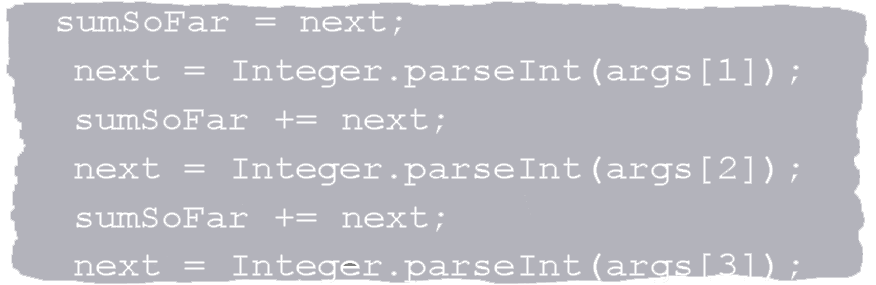
\includegraphics[scale=.3]{what-next-solution.png}   
 \end{center}
  \end{figure}
\end{frame}

\begin{frame}[fragile]{Command-Line Arguments}
 \textbf{Building Blocks of a Program}
 
 \vspace{1pc}
 We will construct the following expressions, which we will use in our FIRST Java program:
 \begin{lstlisting}[numbers=none]
a1 = Integer.parseInt(args[0]); //Read first number
a2 = Integer.parseInt(args[1]); // Read second number
sum = a1 + a2; // add a1 and a2 and assign to sum
a3 = Integer.parseInt(args[2]); // Read third number
sum = sum + a3; // add a3 to sum
a4 = Integer.parseInt(args[3]); // Read fourth number
sum += a4; // Add a4 to sum
System.out.println(sum); //print sum
 \end{lstlisting}
\end{frame}

\begin{frame}{Command-Line Arguments}
 \begin{itemize}
  \item Java application can accept any number of arguments directly from the command-line. 
  \item Users can enter command-line arguments when invoking the application. 
  \item When running the java program with java command, the arguments are provided after the name of the class, separated by space.
 \end{itemize}
\end{frame}

\begin{frame}{Command-Line Arguments}
 Receive Command-line Arguments - Main
 \begin{itemize}
  \item In Java, when you invoke an application, the runtime system passes the command-line arguments to the application's main method as an array of Strings.
 
 \lstinline!public static void main(String[] args)!
 
 \item Each String in the array contains one of the command-line arguments.
 \end{itemize}
\end{frame}

\begin{frame}[fragile]{Command-Line Arguments}
 \begin{block}{Sample Program} 
  \begin{lstlisting}[numbers=none]
class CMDArgs {
    public static void main(String[] args) {
        System.out.println("Hello: " + args[0]);
    }
}
 \end{lstlisting}
 \end{block}
\begin{description}
 \item [Compile] javac  CMDArgs.java
 \item [Run] java  CMDArgs TalentSprint
 \item [Output] Hello TalentSprint
\end{description}
\end{frame}

\begin{frame}{Command-Line Arguments}
\begin{enumerate}
 \item Write a program which accepts two names as input values and  print ``Hello <name1> and <name2>'' as output.
 
 Note: Use command-line arguments

 \item Create a file \lstinline!Wish.java! and pass two command-line arguments. First argument is AM/PM and second argument is your name. Program should  print ``Good Morning <your name>'', if first argument is `AM'.  If the argument is `PM' then it should print ``Good Evening <your name>''.
 \begin{block}{Note}
 If first argument is not equal to ``AM'' or ``PM'' then it should print ``First argument should be either `AM' or `PM' ''. 
 \end{block}
 \end{enumerate}
\end{frame}

\begin{frame}[fragile]{Command-Line Arguments}
 \textbf{Conversion of Command-line Argument}
 \begin{itemize}
  \item If your program needs to support a numeric command-line argument, it must convert a String argument that represents a number, such as "34", to a number.
  \item The following is a code snippet that converts a command-line argument to an integer:
   \begin{lstlisting}[numbers=none]
int firstArg = 0;
if (args.length > 0)
    firstArg = Integer.parseInt(args[0]);
   \end{lstlisting}
 \end{itemize}
 The \lstinline!parseInt()! method in the Integer class throws a \lstinline!NumberFormatException(ERROR)!, if the format of args[0] isn't valid  (not a number).
\end{frame}

\begin{frame}[fragile]{Command-Line Arguments}
 \begin{itemize}
  \item Before using command-line arguments, always check the number of arguments, that too, before accessing the array elements, so that there will be no exception generated.
  \item For example, if your program needs the user to input 5 arguments, then:
  \begin{lstlisting}[numbers=none]
if (args.length != 5) {
    System.out.println("Invalid number of arguments");
    System.out.println("Please enter 5 arguments");
    return;
}
  \end{lstlisting}
 \end{itemize}
\end{frame}

\begin{frame}[fragile]{Command-Line Arguments}
 \begin{block}{Adding Two Values Using Command Line Arguments}
 \begin{lstlisting}[numbers=none]
class SumOfTwoNums {
    public static void main(String[] args) {
        // convert first value into integer
        int firstNum = Integer.parseInt(args0]);		
        // convert second value into integer 
        int secondNum = Integer.parseInt(args[1]);
        int sum = firstNum + secondNum;
        System.out.println("Sum: " + sum);
    }
}
 \end{lstlisting}
 \end{block}
\begin{description}
 \item [Compile] javac SumOfTwoNums.java
 \item [Run] java  SumOfTwoNums 10 20
 \item [Output] Sum: 30
\end{description}
\end{frame}

\begin{frame}[fragile]{Command-Line Arguments}
 Execute the previous program by passing different values:
 
 \vspace{1pc}
 \begin{description}
  \item [1] java SumOfTwoNums 30 40
  \item [2] java SumOfTwoNums 20 30 40
  \item [3] java SumOfTwoNums 30
  \item [4] java SumOfTwoNums 30 A
  \item [5] java SumOfTwoNums abc ABC
 \end{description}
\end{frame}

\begin{frame}[fragile]{Command-Line Arguments}
Try to run the following program and see what happens.
\begin{lstlisting}[numbers=none]
class CMDArgs1 {
    public static void main(String[] args) {
        int intAge = Integer.parseInt(args[1]);
        String strName = args[2];
        System.out.println("Age: " + intAge);
        System.out.println("Name: " + strName);
    }
}
\end{lstlisting}
\end{frame}

\begin{frame}{Command-Line Arguments}
 Possible Errors With Command Line Arguments
 
 \vspace{1pc}
 \begin{description}
  \item [ArrayIndexOutOfBoundsException] If user does not pass sufficient number of values (or) array index is beyond its size.
  \item [NumberFormatException] If user pass alphabets or symbols, where integers are expected.  (or)  while  converting alphabets or symbols to integers.
 \end{description}
\end{frame}

\begin{frame}{Command-Line Arguments}
 \textbf{Operators}
 
 \begin{description}
  \item [Arithmetic Operators] + \hspace{.4pc}- \hspace{.4pc}* \hspace{.4pc}/
  \item [Assignment Operators] = \hspace{.4pc}+= \hspace{.4pc}-= \hspace{.4pc}*= \hspace{.4pc}/=
  \item [Relational Operators] $<$ \hspace{.4pc}$<$= \hspace{.4pc}$>$ \hspace{.4pc}$>$= \hspace{.4pc}== \hspace{.4pc}!=
  \end{description}
  Can you name these operators and operations they perform on operands?
\end{frame}

\begin{frame}[fragile]{Command-Line Arguments}
 \begin{block}{Operators} 
 An operator represents an operation to be performed on the given operands.
 \end{block}
 \begin{block}{Expressions}
  \begin{lstlisting}[numbers=none]
   int sum1 = a1 + a2;
       or
   System.out.println("Sum: " + sum);
  \end{lstlisting}
 \end{block}
An expression is a construct made up of variables, operators, and method invocations, which are constructed according to the syntax of the language, that evaluates to a single value.
 
\end{frame}


\begin{frame}{Command-Line Arguments}
 \begin{figure}[H]
 \begin{center}
   
\includegraphics[scale=.3]{qa.png}   
 \end{center}
  \end{figure}
\end{frame}



\end{document}

